\documentclass[12pt,oneside]{fithesis2}
\usepackage[slovak]{babel}       % Multilingual support
\usepackage[utf8]{inputenc}       % UTF-8 encoding
\usepackage[T1]{fontenc}          % T1 font encoding
\usepackage[                      % A sans serif font that blends well with Palatino
  scaled=0.86
]{berasans}
\usepackage[                      % A tt font if you do not like LM's tt
  scaled=1.03
]{inconsolata}
\usepackage[                      % Clickable links
  plainpages = false,               % We have multiple page numberings
  pdfpagelabels                     % Generate pdf page labels
]{hyperref}
\usepackage{blindtext}            % Lorem ipsum generator
\usepackage{amsmath}

\thesislang{sk}                   % The language of the thesis
\thesistitle{Vyhľadávanie najbližších vektorov s využitím knižnice FLANN}       % The title of the thesis
\thesissubtitle{Bakalárska práca}  % The type of the thesis
\thesisstudent{Tomáš Durčák}          % Your name
\thesiswoman{false}                % Your gender
\thesisfaculty{fi}                % Your faculty
\thesisyear{Jar \the\year}     % The academic term of your thesis defense
\thesisadvisor{RNDr. David Novák, Ph.D.}   % Your advisor

\begin{document}
  \FrontMatter                    % The front matter
    \ThesisTitlePage                % The title page
    \begin{ThesisDeclaration}       % The declaration
      \DeclarationText
      \AdvisorName
    \end{ThesisDeclaration}
    \begin{ThesisThanks}            % The acknowledgements (optional)
      I would like to thank my supervisor\,\dots
    \end{ThesisThanks}
    \begin{ThesisAbstract}          % The abstract
      The aim of the bachelor work is to provide\,\dots
    \end{ThesisAbstract}
    \begin{ThesisKeyWords}          % The keywords
      keyword1, keyword2\,\dots
    \end{ThesisKeyWords}
    \tableofcontents                % The table of contents
%   \listoftables                   % The list of tables (optional)
%   \listoffigures                  % The list of figures (optional)
  
  \MainMatter                     % The main matter
    \chapter{Úvod}          % Chapters
    
    \chapter{Základné pojmy}
    
    	\section{Vektorový priestor}
    Vektorový priestor $ \Omega = D_1D_2. . .D_n $ má dimenziu $n$. Objekt (resp. vektor, resp.bod)  $\mathcal{O} = [a_1, a_2, . . . , a_n] $ patriaci do vektorového priestoru je jednoznačne určeny svojimi súradnicami $ a_i \in D_i, 1 \le i \le n, $ ktorých je práve $n$. Každá jednotlivá dimenzia má svoju doménu $D_i$ - množinu hodnôt (resp. vlastností), ktoré môže prislušná vektorová súradnica nadobúdať.
    	
    Vektorový priestor $\Omega$, definujeme nad určitým poľom $\mathbf{P} $, s význačným prvkom $\mathbf{0}$ a dvomi binárnymi operáciami, sčítaním $+ : \Omega \times \Omega \rightarrow \Omega $  a násobením $. : \mathbf{P}  \times \Omega \rightarrow \Omega$, takými že platí: 
     
\begin{equation*}
\forall u,v,w \in \Omega : (u + v)+w = u+(v+w) 
\end{equation*}
\begin{equation*}
\exists\mathbf{0} \in \Omega : u+\mathbf{0} = \mathbf{0}+u = u
\end{equation*}
\begin{equation*}
\forall u \in \Omega \; \exists \; u \in \Omega : u+(-u)  = \mathbf{0}
\end{equation*}
\begin{equation*}
\forall a,b \in \mathbf{P} \; \exists \; u \in \Omega : (a.b).u = a.(b.u) 
\end{equation*}
\begin{equation*}
\forall u \in \Omega : 1.u=u  \textrm{ kde } 1 \in \mathbf{P}  \textrm{ je jednotkový prvok z } \mathbf{P} 
\end{equation*}
\begin{equation*}
\forall a,b \in \mathbf{P} \; \exists \;u \in \Omega : (a+b).u = a.u + b.u 
\end{equation*}
\begin{equation*}
\forall a \in \mathbf{P} \; \exists \;u,v \in \Omega : a.(u+v) = a.u + a.v 
\end{equation*} \\
\textbf{Poznámka:} Vektorový podpriestor je tiež vektorový priestor.

\begin{figure}
  \centering
  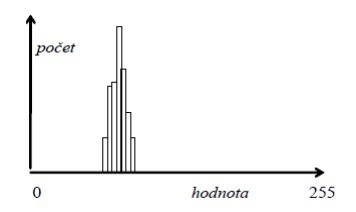
\includegraphics[width=6cm]{gis_histogram_obrazu.png}
  \caption{Histogram farieb so siedmimi farebnými odtieňmi.}
  \label{fig:triangle}
\end{figure}  

\textbf{Príklad:}
Obrázok (resp. jeho histogram farieb) može byť vektorom vo vektorovom priestore a mať súradnice podľa počtu pixelov z každého farebného odtieňu.
Potom vektor z histogramu farieb je:
\begin{equation}
\{(\alpha_1,\beta_1),...(\alpha_M,\beta_M)\}
\end{equation}
kde $M$ je počet farebných odtieňov. \\
Iným príkladom môže byť dokument reprezentovaný ako
vektor v $m$-rozmernom priestore príznakov, ktoré zodpovedajú jednotlivým slovám – tzv.termom. Množina $n$ dokumentov je reprezentovaná ako matica $n\times m$. Neplnovýznamové slová (pomocne slovesá, spojky...) sa zvyčajne odstránia.


    \section{Metrický priestor}
    
    Metrický priestor je množina, na ktorej je definovaná vzdialenosť pre všetky prvky z množiny. Táto vzdialenosť sa nazýva metrika. Metriku môžme definovať ako funkciu, ktorá určuje vzdialenosť medzi dvomi objektami. \\ \\
    \textbf{Definícia:} Nech $X\neq 0$ je množina. Definujme zobrazenie \\ $d: X \times X \rightarrow R $, ktoré spĺňa nasledujúce vlastnosti:
    \begin{align*}
    \textrm{ Pre všetky } x,y,z \in X \qquad d(x,x) &= 0 \\
    d(x,y) &\textgreater 0 \qquad x\neq y \\
    d(x,y) &= d(y,x) \\
    d(x,z) + d(z,y) &\geq d(x,y)
    \end{align*}
    
    Množinu \textbf{$X$} nazývame \textbf{základnou množinou}, zobrazenie $d$ \textbf{metrikou} a usporiadanu dvojicu $(X,d)$ \textbf{metrickým priestorom}.
    V tej istej množine možme definovať rôzne metriky. Metrika $d$ musí byť vždy nezáporná. \\ \\
    \textbf{Príklad:} 
    Vzdialenosť dvoch bodov na priamke v $ \mathbf{R} \quad d=|x-y| $ alebo v rovine v
     $\mathbf{R^2} \quad d = \sqrt{(x_1-y_1)^2+(x_2-y_2)^2}$.
    
	\section{Vzdialenostné funkcie}
	Vzdialenostné funcie predstavuju hlavný spôsob určenia blízkosti alebo podobnosti dvoch objektov v určitej doméne. Táto vzdialenosť može byť definovaná rôzne. Najčastejšie v zavislosti od použitého datového typu alebo účelu aplikácie.
	Vzdialenostné funkcie rozdeľujeme na dva zakladne typy podľa charakteru ich návratovej hodnoty:
	\begin{itemize}
	\item \textbf{diskrétne --} vracajú len vopred určenú množinu hodnôt malého rozsahu, napr. 	     len hodnotu $1$ alebo $-1$
	\item \textbf{spojité --} rozsah vrátenej množiny hodnôt je veľmi veľký alebo aj nekonečno, 		napr. hodnoty z intervalu $[0,1]$
	\end{itemize}
	Ďalej si popíšeme najčastejšie používané vzdialenostné funkcie. Jednu z nich budeme používať aj v testovaní a porovnávaní testovaných knižníc.
\subsection{Minkowského vzdialenosť}
Minkowského vzdialenosť je generalizovaná metrika, ktorá zahŕňa tzv. $L_p$ metriky v zovšebecnenej forme. Minkowskí ju definoval takto: 
\begin{equation*}
L_p((x_1,...,x_n),(y_1,...,y_n))=\sqrt[p]{(\sum\limits_{i=1}^n \mid x_i-y_i \mid^p )}
\end{equation*}
Rovnica udáva vzdialenosť medzi dvomi objektami v $n$-dimenzionalnom priestore pre $p\geq 1$ (ak by bolo $p \textless 1$ nešlo by o metriku). \\
	\begin{figure}
  		\centering
  		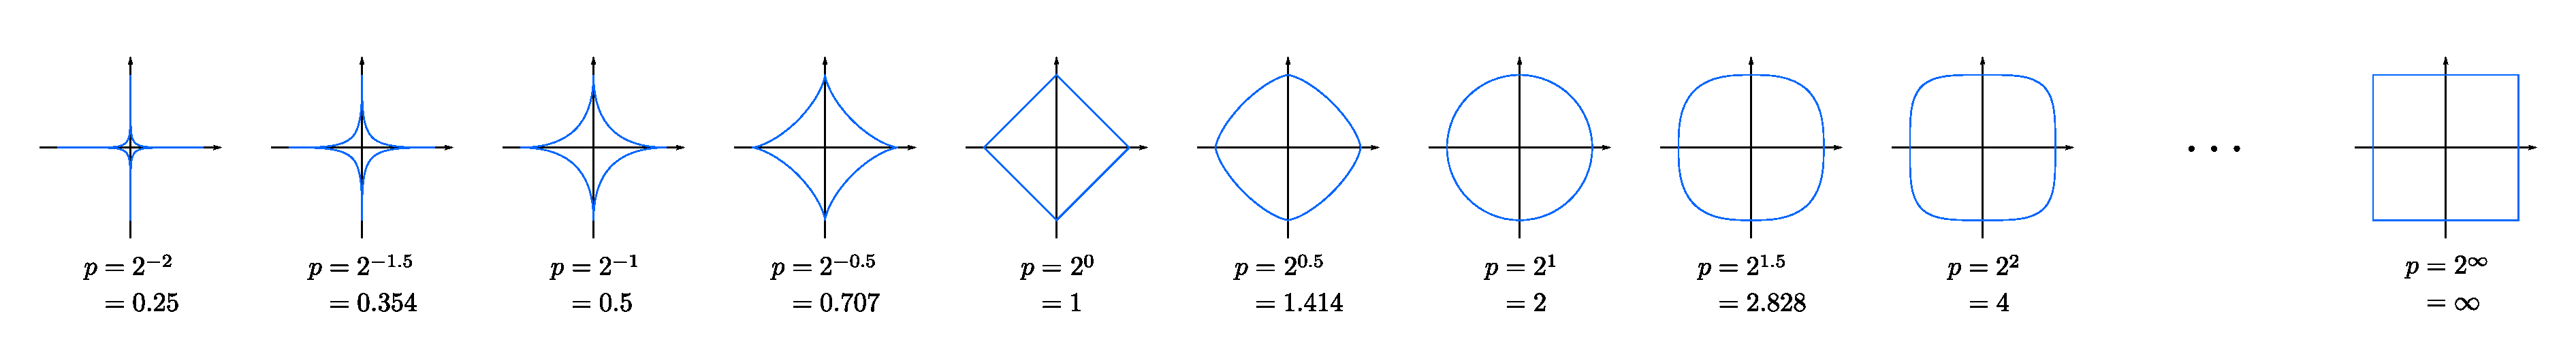
\includegraphics[width=14cm]{obr/lp.eps}
  		\caption{Znázornenie $L_p$- metrik v $R^2$ podľa parametra p}
  		\label{fig:triangle}
	\end{figure}  

Medzi najznámejšie a napoužívanejšie metriky patria:
\begin{itemize}
\item $L_1$ -- Manhattanská metrika vyjadruje najkratšiu vzdialenosť, ktoru musíme prejsť aby sme sa v meste dostali z jedneho bodu do druhého. Je pomenovaná podľa pravouhélo systému ulíc v meste New York.
\item $L_2$ -- Eklidovská metrika vyjadruje najkračšiu vzdušnú vzdialenosť medzi dvomi objektmi. $L_2$ je použitá aj pri testoch.
\item $L_\infty $ -- Čebyševova metrika, nazýva sa tiež maximálna alebo šachovnicová vzdialenosť, pretože na šachovnici, je to minimalny počet ťahov potrebných na prejdenie kráľom z jedného štvorca na iný.
\end{itemize}
   \section{Vyhľadávanie v metrických a vektorových priestoroch}
   Základnou charakteristikou vyhľadávania vo vektorových a metrických priestoroch je neurčitosť. Týka sa to hlavne problému \textbf{Najdenia najbližšieho suseda} (ang. Nearest neighbor search). Tento problém obecne definujeme takto: \\
   Je daná množina bodov $P=\{p_1,...,p_n\}$ v priestore $X$ a dotazované body $q \in M$, nájdite najbližšie body z $P$ ku $q$.\\
   Pod pojmom \textbf{najbližši sused} rozumieme objekt alebo bod podobný dotazovanému bodu. Nepožadujeme aby boli vysledky vyhľadávania vždy na 100\% presné, ale aby výpočet skončil v čo najkratšom čase.
   Pred vyhľadávaním sa musíme rozhodnúť, ako chceme určovať blízkosť objektov, akú metriku použijeme. V našich testoch bola použitá $L_2$ metrika, čiže klasická Euklidovská metrika, ktorá je vhodná pre husto vzorkované dáta. Ďalej sa musíme rozhodnúť, koľko najbližšich susedov budeme hľadať. Existujú 3 základné druhy dotazov:
   \begin{itemize}
   \item \textbf{Dotaz na najbližšieho suseda}- hľadáme najližší najpodobnejší objekt k dotazu, výsledkom je 1 objekt ku každému dotazu.
   
   \textbf{Definícia:}
   \begin{equation*}
   NN(q)=\{x \in X, \forall y \in X| d(q,x)\leq d(q,y) \}
   \end{equation*}
Výsledkom je bod $x$, ktorého vzdialenosť od dotazu $q$ je najmenšia spomedzi všetkých bodov z množiny $X$.
   \item \textbf{Dotaz na k-najbližších susedov}- niekedy nám nemusí stačiť len 1 najbližší objekt, preto hľadáme $k$ susedov, ktoré sú mu podobné.
   
   \textbf{Definícia:}
   \begin{equation*}
   kNN(q)=\{A|A \subseteq X,|A|=k,\forall x \in A,\forall y \in X - A,d(q,x)\leq d(q,y)\}
   \end{equation*}    
   \item \textbf{Rozsahový dotaz}- použijeme, keď chceme nájsť všetkych najbližších susedov, ktorý su od dotazovaného bodu $q$ vzdialený maximálne zvolenú hodnotu $r$ (polomer vyhľadávania).
   
   \textbf{Definícia:} %R(q,r)=\{ x \in X|d(q,x)\leq r \}
   \begin{equation*} 
  rNN(q,X,r)=\{ x \in X|d(q,x)\leq r \}
   \end{equation*}  
   \end{itemize}
   
	\begin{figure}
  		\centering
  		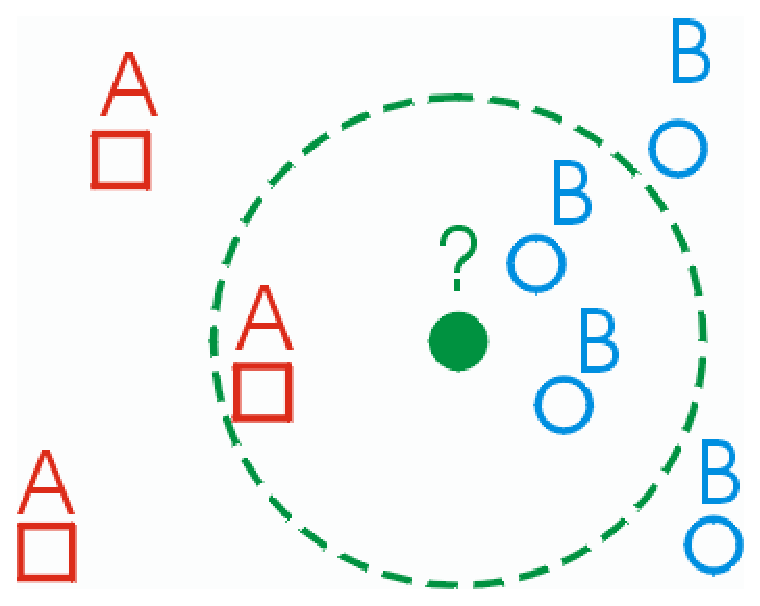
\includegraphics[width=6.5cm]{obr/Image25.eps}
  		\caption{Znázornenie $kNN$ a $rNN$ v $L_2$-metrike}
  		\label{fig:triangle}
	\end{figure}  
   
   
   
    \chapter{Výsledky testov}
    
    \chapter{Záver}

    \chapter{First appendix}        % Appendices

    \chapter{Another appendix}

    % Bibliography goes here
    % Index goes here (optional)
\end{document}
